\documentclass{standalone}
\usepackage{tikz}
\usetikzlibrary{patterns, positioning}


\begin{document}
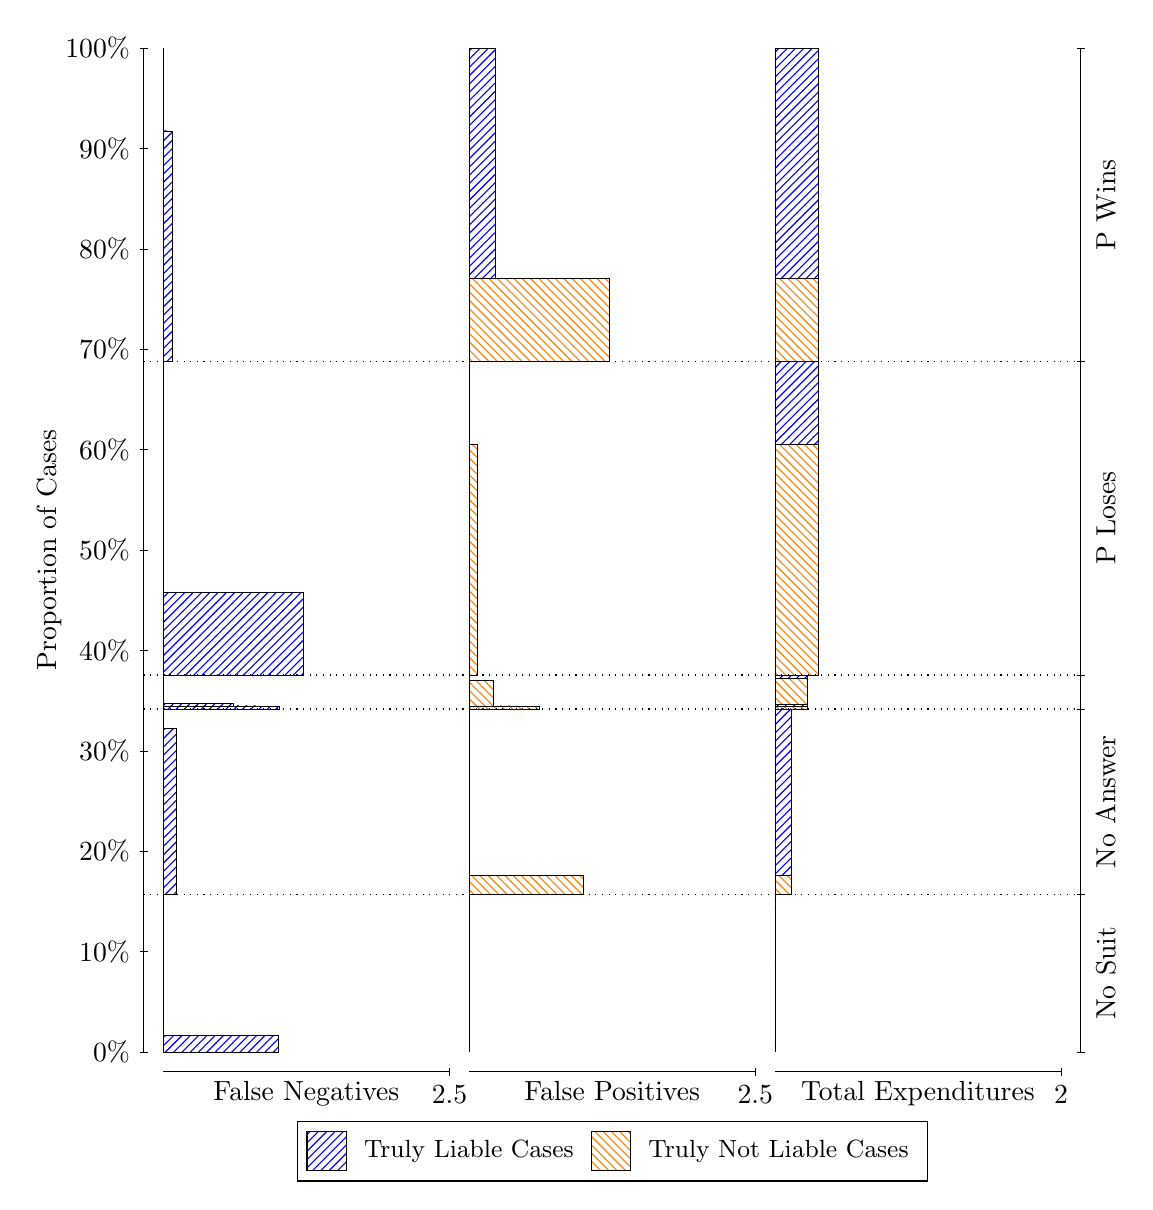
\begin{tikzpicture}
\draw[black, very thin] (1.5,1.75) -- (1.5,14.5);
\node[rotate=90, text=black, anchor=center] at (0.3, 8.125) {Proportion of Cases};
\draw[black, very thin] (1.45,1.75) -- (1.55,1.75);
\node[text=black, anchor=east] at (1.45, 1.75) {0\%};
\draw[black, very thin] (1.45,3.025) -- (1.55,3.025);
\node[text=black, anchor=east] at (1.45, 3.025) {10\%};
\draw[black, very thin] (1.45,4.3) -- (1.55,4.3);
\node[text=black, anchor=east] at (1.45, 4.3) {20\%};
\draw[black, very thin] (1.45,5.575) -- (1.55,5.575);
\node[text=black, anchor=east] at (1.45, 5.575) {30\%};
\draw[black, very thin] (1.45,6.85) -- (1.55,6.85);
\node[text=black, anchor=east] at (1.45, 6.85) {40\%};
\draw[black, very thin] (1.45,8.125) -- (1.55,8.125);
\node[text=black, anchor=east] at (1.45, 8.125) {50\%};
\draw[black, very thin] (1.45,9.4) -- (1.55,9.4);
\node[text=black, anchor=east] at (1.45, 9.4) {60\%};
\draw[black, very thin] (1.45,10.675) -- (1.55,10.675);
\node[text=black, anchor=east] at (1.45, 10.675) {70\%};
\draw[black, very thin] (1.45,11.95) -- (1.55,11.95);
\node[text=black, anchor=east] at (1.45, 11.95) {80\%};
\draw[black, very thin] (1.45,13.225) -- (1.55,13.225);
\node[text=black, anchor=east] at (1.45, 13.225) {90\%};
\draw[black, very thin] (1.45,14.5) -- (1.55,14.5);
\node[text=black, anchor=east] at (1.45, 14.5) {100\%};

\draw[black, very thin] (13.4,1.75) -- (13.4,14.5);
\draw[black, very thin] (13.35,1.75) -- (13.45,1.75);
\node[anchor=west] at (13.35, 1.75) {};
\draw[black, very thin] (13.35,3.7486) -- (13.45,3.7486);
\node[anchor=west] at (13.35, 3.7486) {};
\draw[black, very thin] (13.35,6.1064) -- (13.45,6.1064);
\node[anchor=west] at (13.35, 6.1064) {};
\draw[black, very thin] (13.35,6.5373) -- (13.45,6.5373);
\node[anchor=west] at (13.35, 6.5373) {};
\draw[black, very thin] (13.35,10.519) -- (13.45,10.519);
\node[anchor=west] at (13.35, 10.519) {};
\draw[black, very thin] (13.35,14.5) -- (13.45,14.5);
\node[anchor=west] at (13.35, 14.5) {};

\draw[black, very thin, pattern color=blue, pattern=north east lines] (1.75,1.75) rectangle (3.2033,1.9603);
\draw[black, very thin, pattern color=orange, pattern=north west lines] (1.75,1.9603) rectangle (1.75,3.7486);
\draw[black, very thin, pattern color=blue, pattern=north east lines] (1.75,3.7486) rectangle (1.9135,5.864);
\draw[black, very thin, pattern color=orange, pattern=north west lines] (1.75,5.864) rectangle (1.75,6.1064);
\draw[black, very thin, pattern color=blue, pattern=north east lines] (1.75,6.1064) rectangle (3.2215,6.1409);
\draw[black, very thin, pattern color=blue, pattern=north east lines] (1.75,6.1409) rectangle (2.9308,6.1444);
\draw[black, very thin, pattern color=blue, pattern=north east lines] (1.75,6.1444) rectangle (2.6402,6.1743);
\draw[black, very thin, pattern color=orange, pattern=north west lines] (1.75,6.1743) rectangle (1.75,6.5373);
\draw[black, very thin, pattern color=blue, pattern=north east lines] (1.75,6.5373) rectangle (3.5303,7.5895);
\draw[black, very thin, pattern color=orange, pattern=north west lines] (1.75,7.5895) rectangle (1.75,10.519);
\draw[black, very thin, pattern color=blue, pattern=north east lines] (1.75,10.519) rectangle (1.859,13.448);
\draw[black, very thin, pattern color=orange, pattern=north west lines] (1.75,13.448) rectangle (1.75,14.5);
\draw[black, very thin, pattern color=orange, pattern=north west lines] (5.6333,1.75) rectangle (5.6333,3.5383);
\draw[black, very thin, pattern color=blue, pattern=north east lines] (5.6333,3.5383) rectangle (5.6333,3.7486);
\draw[black, very thin, pattern color=orange, pattern=north west lines] (5.6333,3.7486) rectangle (7.0867,3.991);
\draw[black, very thin, pattern color=blue, pattern=north east lines] (5.6333,3.991) rectangle (5.6333,6.1064);
\draw[black, very thin, pattern color=orange, pattern=north west lines] (5.6333,6.1064) rectangle (6.5235,6.1363);
\draw[black, very thin, pattern color=orange, pattern=north west lines] (5.6333,6.1363) rectangle (6.2328,6.144);
\draw[black, very thin, pattern color=orange, pattern=north west lines] (5.6333,6.144) rectangle (5.9422,6.4694);
\draw[black, very thin, pattern color=blue, pattern=north east lines] (5.6333,6.4694) rectangle (5.6333,6.5373);
\draw[black, very thin, pattern color=orange, pattern=north west lines] (5.6333,6.5373) rectangle (5.7423,9.4665);
\draw[black, very thin, pattern color=blue, pattern=north east lines] (5.6333,9.4665) rectangle (5.6333,10.519);
\draw[black, very thin, pattern color=orange, pattern=north west lines] (5.6333,10.519) rectangle (7.4137,11.571);
\draw[black, very thin, pattern color=blue, pattern=north east lines] (5.6333,11.571) rectangle (5.9603,14.5);
\draw[black, very thin, pattern color=orange, pattern=north west lines] (9.5167,1.75) rectangle (9.5167,3.5383);
\draw[black, very thin, pattern color=blue, pattern=north east lines] (9.5167,3.5383) rectangle (9.5167,3.7486);
\draw[black, very thin, pattern color=orange, pattern=north west lines] (9.5167,3.7486) rectangle (9.721,3.991);
\draw[black, very thin, pattern color=blue, pattern=north east lines] (9.5167,3.991) rectangle (9.721,6.1064);
\draw[black, very thin, pattern color=orange, pattern=north west lines] (9.5167,6.1064) rectangle (9.9254,6.1363);
\draw[black, very thin, pattern color=blue, pattern=north east lines] (9.5167,6.1363) rectangle (9.9254,6.1662);
\draw[black, very thin, pattern color=orange, pattern=north west lines] (9.5167,6.1662) rectangle (9.9254,6.4993);
\draw[black, very thin, pattern color=blue, pattern=north east lines] (9.5167,6.4993) rectangle (9.9254,6.5373);
\draw[black, very thin, pattern color=orange, pattern=north west lines] (9.5167,6.5373) rectangle (10.062,9.4665);
\draw[black, very thin, pattern color=blue, pattern=north east lines] (9.5167,9.4665) rectangle (10.062,10.519);
\draw[black, very thin, pattern color=orange, pattern=north west lines] (9.5167,10.519) rectangle (10.062,11.571);
\draw[black, very thin, pattern color=blue, pattern=north east lines] (9.5167,11.571) rectangle (10.062,14.5);
\draw[black, dotted] (1.5,3.7486) -- (13.4,3.7486);
\draw[black, dotted] (1.5,6.1064) -- (13.4,6.1064);
\draw[black, dotted] (1.5,6.5373) -- (13.4,6.5373);
\draw[black, dotted] (1.5,10.519) -- (13.4,10.519);
\draw[black, very thin] (1.75,1.5) -- (5.3833,1.5);
\node[text=black, anchor=north] at (3.5667, 1.5) {False Negatives};
\draw[black, very thin] (5.3833,1.45) -- (5.3833,1.55);
\node[text=black, anchor=north] at (5.3833, 1.45) {2.5};

\draw[black, very thin] (5.6333,1.5) -- (9.2667,1.5);
\node[text=black, anchor=north] at (7.45, 1.5) {False Positives};
\draw[black, very thin] (9.2667,1.45) -- (9.2667,1.55);
\node[text=black, anchor=north] at (9.2667, 1.45) {2.5};

\draw[black, very thin] (9.5167,1.5) -- (13.15,1.5);
\node[text=black, anchor=north] at (11.333, 1.5) {Total Expenditures};
\draw[black, very thin] (13.15,1.45) -- (13.15,1.55);
\node[text=black, anchor=north] at (13.15, 1.45) {2};

\node[text=black, centered, rotate=90] at (13.72, 2.7493) {No Suit};
\node[text=black, centered, rotate=90] at (13.72, 4.9275) {No Answer};

\node[text=black, centered, rotate=90] at (13.72, 8.528) {P Loses};
\node[text=black, centered, rotate=90] at (13.72, 12.509) {P Wins};

\draw (7.449999999999999,1.5) node[draw=none] (baseCoordinate) {};
\begin{scope}[align=center]
        \matrix[scale=0.5, draw=black, below=0.5cm of baseCoordinate, nodes={draw}, column sep=0.1cm]{
            \node[rectangle, draw, minimum width=0.5cm, minimum height=0.5cm, pattern color=blue, pattern=north east lines] {}; &
            \node[draw=none, font=\small, text=black] (B) {Truly Liable Cases}; &
            \node[rectangle, draw, minimum width=0.5cm, minimum height=0.5cm, pattern color=orange, pattern=north west lines] {}; &
            \node[draw=none, font=\small, text=black] (B) {Truly Not Liable Cases}; \\
            };
\end{scope}

\end{tikzpicture}
\end{document}